% A circular diagram of a TeX workflow
% Author: Stefan Kottwitz
% https://www.packtpub.com/hardware-and-creative/latex-cookbook
\documentclass[border=10pt]{standalone}
\usepackage{tikz} 
\usetikzlibrary{shapes,arrows}
%\usepgfplotslibrary{external} 
%\tikzexternalize 
\usepackage{sansmath}
\sansmath

\tikzstyle{block1} = [rectangle, draw,fill=green!80!black!20, 
text width=8em, text centered, rounded corners, minimum height=4em]
\tikzstyle{block} = [rectangle, draw, 
text width=8em, text centered, rounded corners, minimum height=4em]
\tikzstyle{line} = [draw, -latex']

\begin{document}
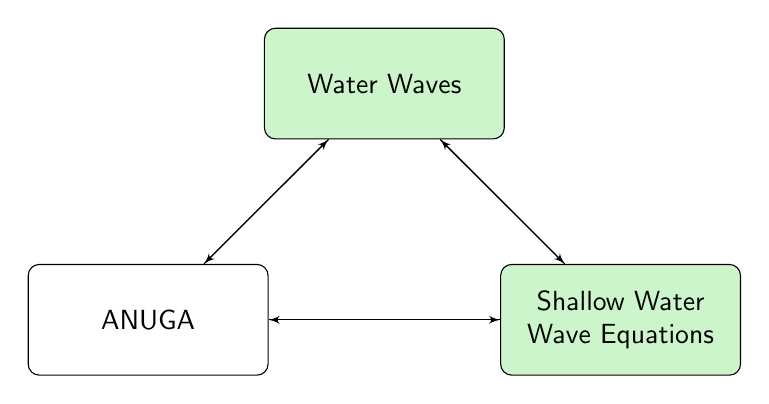
\begin{tikzpicture} 
\fontfamily{cmss}
 \node [block1] (PP) {Water Waves};
 \node [block1,below of=PP,right of=PP, node distance=3cm](MM) {Shallow Water Wave Equations};
 \node [block,left of= PP,below of=PP, node distance=3cm](CP) {ANUGA};
 \path [line] (PP) -> (MM);
 \path [line] (MM) -> (PP);
 \path [line] (MM) -> (CP);
 \path [line] (CP) -> (MM);
 \path [line] (CP) -> (PP);
 \path [line] (PP) -> (CP);
\end{tikzpicture} 
\end{document}